\documentclass[output=paper,colorlinks,citecolor=brown]{langscibook}
\ChapterDOI{10.5281/zenodo.15006601}
\author{Keiko Hirano\orcid{}\affiliation{The University of Kitakyushu, Japan}}
\title{A directional shift in linguistic change: A longitudinal study on English-speaking expatriates in Japan}

\abstract{This paper attempts to demonstrate that the direction of linguistic change in a dialect contact environment can shift over time. The analysis reports on the linguistic change in an English-speaking expatriate community in Japan in which dialect contact (\citealt{Britain2018, Trudgill1986, Trudgill2004}) occurs among different varieties of English. Speakers’ choice of possessive verbs (\textit{have got}, \textit{have}, and \textit{got}) and obligatory verbs (\textit{must, have got to, have to}, and \textit{got to}) is examined. This longitudinal study is based on three sets of linguistic data: (1) a corpus of English-language conversations collected in 2000 from young British and American English speakers who had recently arrived in Japan [Data 1], (2) a corpus collected in 2001 from the same speakers after they had lived in Japan for a year [Data 2], and (3) a corpus collected in and after 2018 from British and Americans who had worked and lived in Japan for an average of 20 years [Data 3]. The analysis of the use of possessive verbs suggests that the British English speakers used more typically “British” grammatical constructions (\textit{have got}) in Data 2 (one year after their arrival in Japan), while the American English speakers maintained their use of more typically “American” constructions (\textit{have} and \textit{got}) in Data 2. However, the analysis of Data 3 (after living in Japan for an average of 20 years) suggests an alteration in the direction of this linguistic change. Both the British and American speakers adopted the use of verbs that had strong associations with the other nationality’s English style. A similar tendency was observed in terms of the choice of verbs of obligation. These results indicate that the direction of linguistic change in a dialect contact environment is not always unidirectional but may shift over the long term. These linguistic changes appear to be the outcome of “long-term accommodation” \citep{Trudgill1986} in which speakers adopt certain linguistic features in another variety of the same language and incorporate these features permanently.}

\IfFileExists{../localcommands.tex}{
  \addbibresource{../localbibliography.bib}
  \usepackage{tabularx,multicol}
%\usepackage{multirow}
\usepackage{subcaption}
\usepackage{url}
\urlstyle{same}

\usepackage{datetime}
\usepackage{enumitem}
\usepackage{langsci-optional}
\usepackage{langsci-lgr}
\usepackage{langsci-branding}

\usepackage{longtable}
\usepackage{xltabular}
\usepackage[linguistics, edges]{forest}
\usepackage{pgfplots}
\pgfplotsset{compat=1.18}
\usetikzlibrary{patterns, tikzmark}
\usepackage{pgfplotstable}
\usepgfplotslibrary{colorbrewer}
\usepackage{listings}
\lstset{basicstyle=\ttfamily,keywordstyle=\normalfont,language=,breaklines=true}

\usepackage{siunitx}
\sisetup{group-digits=none, detect-all=true}

\usepackage{langsci-gb4e}

  \makeatletter
\let\thetitle\@title
\let\theauthor\@author
\makeatother

% Use this Chinese font shipped with TeX Live instead of Source Han, because
% it is more portable/leightweight. Install the "fandol" package from CTAN to
% automatically get this font.
\newfontfamily{\ChineseFandolSong}{FandolSong-Regular.otf}

  %% hyphenation points for line breaks
%% Normally, automatic hyphenation in LaTeX is very good
%% If a word is mis-hyphenated, add it to this file
%%
%% add information to TeX file before \begin{document} with:
%% %% hyphenation points for line breaks
%% Normally, automatic hyphenation in LaTeX is very good
%% If a word is mis-hyphenated, add it to this file
%%
%% add information to TeX file before \begin{document} with:
%% %% hyphenation points for line breaks
%% Normally, automatic hyphenation in LaTeX is very good
%% If a word is mis-hyphenated, add it to this file
%%
%% add information to TeX file before \begin{document} with:
%% \include{localhyphenation}
\hyphenation{
    a-na-ly-sis
    ap-proach-es
    ar-che-o-log-i-cal
    Ar-khan-gelsk
    be-schrei-ben
    Buch-holtz
    Che-lya-binsk
    con-so-nant
    dia-lect
    dia-lect-ology
    Di-a-lekt-for-schung
    Dia-lekt-for-schung
    East-pha-lian
    För-der-ung
    Ge-mein-schaft-lich-keits-ent-wür-fe
    his-tor-i-cal
    Hok-kai-do
    ja-pa-nese
    Ja-pa-nese
    Ka-go-shi-ma
    Ka-li-nin-grad
    Knja-zev
    Ma-kro-be-reich
    Ma-lay-sia
    mor-pho-log-i-cal
    Mos-cow
    Nef-te-yu-gansk
    non-mobile
    nu-cle-ar
    ös-ter-rei-chi-sche
    par-a-digm
    per-zep-ti-ons-lin-gu-is-ti-sche
    plu-ri-zen-tri-schen
    quick-ly
    Reich
    Sax-on
    Schrö-der
    sear-ching
    ste-reo-type
    strength-en-ing
    strong-est
    Stutt-gart
    su-pra-seg-men-tal
    teach-er
    to-po-gra-phy
    To-ron-to
    tra-di-tion-al
    ul-ti-mate-ly
    Um-gangs-spra-che
    Volks-kun-de
    vor-zu-stel-len
    wheth-er
    Wie-sing-er
    with-in
    Wort-at-las
}

\hyphenation{
    a-na-ly-sis
    ap-proach-es
    ar-che-o-log-i-cal
    Ar-khan-gelsk
    be-schrei-ben
    Buch-holtz
    Che-lya-binsk
    con-so-nant
    dia-lect
    dia-lect-ology
    Di-a-lekt-for-schung
    Dia-lekt-for-schung
    East-pha-lian
    För-der-ung
    Ge-mein-schaft-lich-keits-ent-wür-fe
    his-tor-i-cal
    Hok-kai-do
    ja-pa-nese
    Ja-pa-nese
    Ka-go-shi-ma
    Ka-li-nin-grad
    Knja-zev
    Ma-kro-be-reich
    Ma-lay-sia
    mor-pho-log-i-cal
    Mos-cow
    Nef-te-yu-gansk
    non-mobile
    nu-cle-ar
    ös-ter-rei-chi-sche
    par-a-digm
    per-zep-ti-ons-lin-gu-is-ti-sche
    plu-ri-zen-tri-schen
    quick-ly
    Reich
    Sax-on
    Schrö-der
    sear-ching
    ste-reo-type
    strength-en-ing
    strong-est
    Stutt-gart
    su-pra-seg-men-tal
    teach-er
    to-po-gra-phy
    To-ron-to
    tra-di-tion-al
    ul-ti-mate-ly
    Um-gangs-spra-che
    Volks-kun-de
    vor-zu-stel-len
    wheth-er
    Wie-sing-er
    with-in
    Wort-at-las
}

\hyphenation{
    a-na-ly-sis
    ap-proach-es
    ar-che-o-log-i-cal
    Ar-khan-gelsk
    be-schrei-ben
    Buch-holtz
    Che-lya-binsk
    con-so-nant
    dia-lect
    dia-lect-ology
    Di-a-lekt-for-schung
    Dia-lekt-for-schung
    East-pha-lian
    För-der-ung
    Ge-mein-schaft-lich-keits-ent-wür-fe
    his-tor-i-cal
    Hok-kai-do
    ja-pa-nese
    Ja-pa-nese
    Ka-go-shi-ma
    Ka-li-nin-grad
    Knja-zev
    Ma-kro-be-reich
    Ma-lay-sia
    mor-pho-log-i-cal
    Mos-cow
    Nef-te-yu-gansk
    non-mobile
    nu-cle-ar
    ös-ter-rei-chi-sche
    par-a-digm
    per-zep-ti-ons-lin-gu-is-ti-sche
    plu-ri-zen-tri-schen
    quick-ly
    Reich
    Sax-on
    Schrö-der
    sear-ching
    ste-reo-type
    strength-en-ing
    strong-est
    Stutt-gart
    su-pra-seg-men-tal
    teach-er
    to-po-gra-phy
    To-ron-to
    tra-di-tion-al
    ul-ti-mate-ly
    Um-gangs-spra-che
    Volks-kun-de
    vor-zu-stel-len
    wheth-er
    Wie-sing-er
    with-in
    Wort-at-las
}

  \togglepaper[1]%%chapternumber
}{}

\begin{document}
\maketitle
\label{chap:hirano}
\shorttitlerunninghead{A directional shift in linguistic change}%%use this for an abridged title in the page headers
\graphicspath{{figures/hirano}}



\section{Introduction}
\label{sec:hirano:1}%1

This paper attempts to demonstrate that the direction of linguistic change in a dialect contact environment can shift over time. This provisional analysis reports on linguistic change that occurs in an English-speaking expatriate community in Japan in which dialect contact (\citealt{Britain2018, Trudgill1986, Trudgill2004}) among English varieties occurs by comparing corpus data from 2000 (Data~1) and 2001 (Data~2) (\citealt{Hirano2013, Hirano2016, HiranoBritain2016, HiranoBritain2020}) with more recent data (Data~3). Speakers’ choice of possessive verbs (\textit{have got}, \textit{have}, and \textit{got}) (\citealt{Hirano2016, HiranoBritain2020}), as indicated in example \REF{ex:hirano:1}, and obligatory verbs (\textit{must, have got to, have to}, and \textit{got to}) (\citealt{HiranoBritain2016, HiranoBritain2020}), as indicated in example \REF{ex:hirano:2}, are examined. From a total of 26 hours of speech collected from 40 native speakers of English (NSsE) from the United Kingdom (UK) and the United States (US), 820 tokens of verbs of possession and 379 tokens of verbs of obligation were extracted.

\ea%1
    \label{ex:hirano:1}
\ea I\textit{’ve got} an elder sister.
\ex I \textit{have} an apartment.
\ex You \textit{got} the West Coast beaches for surfing.
\z
\z

\ea%2
    \label{ex:hirano:2}
\ea We \textit{must} do it like every … three or four months.
\ex I\textit{’ve got to} go to school.
\ex You \textit{have to} have a steady hand.
\ex You \textit{got to} start from somewhere.
\z
\z

The analysis revealed that the directions of linguistic change from Data 1 to Data 2 and those from Data 2 to Data 3 were not identical. This study reveals that a linguistic change which takes place in a long-term dialect contact environment does not necessarily continue to proceed unidirectionally, but may shift in the course of long-term change.

The discussion section attempts to interpret the results of the analyses using the concept of levelling, one of the processes that occurs when a new dialect is created as a result of dialect contact, and the theory of long-term accommodation. Levelling is the eradication of minority or marked variants in a mixed dialect environment (\cites[149--150]{Britain2018}[98--102]{Trudgill1986}). Long-term accommodation occurs as a result of repeated short-term accommodation (\citealt{Coupland1984, GilesPowesland1975}) on a long-term basis towards certain features of specific varieties of the same language \citep[11--21]{Trudgill1986}. This paper explores whether one of these theories can explain the process of the change observed in the use of verbs of possession and obligation induced by dialect contact with speakers of different English varieties in Japan.

\section{The community of native speakers of English} \label{sec:hirano:2}

The NSsE working in Japan range from those who stay in Japan for one to several years as assistant language teachers on the Japan Exchange and Teaching (JET) Programme, or as English teachers in private language schools, to those who stay for several years or several decades as university teachers and researchers or for the purpose of business. The JET Programme employs young university graduates from overseas on fixed-term contracts, and approximately 5,700 people from 57 countries participated in the JET Programme from 2019 to 2020 (\citealt{CouncilofLocalAuthoritiesforInternationalRelations2021}). As of December 2019, there were approximately three million foreign residents in Japan, of which over 430,000 were from major English\hyp speaking countries (\citealt{eStat2021}). Here, “major English-speaking countries” implies those countries where English is used as the first language or one of the official languages and from where over 1000 people resided in Japan as of December 2019. They include, in the order of the largest number of residents, the Philippines, the U.S., India, the U.K., Australia, Canada, New Zealand, Nigeria, Singapore, Ghana, Ireland, and South Africa. These residents engage in a wide variety of social interactions and communication with speakers of their own English dialect, speakers of different English varieties, and non-native speakers of English including Japanese; they are constantly in dialect and language contact situations on a daily basis over a long period of time.

\section{Linguistic variables} \label{sec:hirano:3}%3. /
\subsection{Verbs of possession} %3.1
\label{sec:hirano:3.1}

One of the two linguistic variables for this paper includes the verbs of possession: \textit{have got}, \textit{have}, and \textit{got}. The oldest variants of the possessive verb, \textit{have}, are believed to have their origins in the late tenth century, and \textit{got} is believed to have been added in around the sixteenth century. This resulted in the construction \textit{have got}, which had the same function as \textit{have}. \textit{Got} was the last variant to appear. Presently, \textit{have got} is considered informal, and \textit{got} is considered even more informal. \textit{Got} has been frequently used in American English from the mid-nineteenth century onwards (\cites[207--208]{Kroch1989}[489]{Lorenz2016}[532--534]{Tagliamonte2003}[146--147]{Tagliamonte2013a}[141--142]{Tagliamonte2013b}).

Further, \textit{have got} is characteristic of British English and is used more frequently than \textit{have}; \textit{got} is used less frequently. In the UK, younger speakers tend to use \textit{have got} more frequently than older speakers. On the other hand, \textit{have} and \textit{got} are expressions characteristic of North American English. \textit{Have} is the most frequently used form and \textit{got} is particularly strongly associated with North American English. Further, in North American English, younger people tend to use \textit{have} more often than older people (\cites[25--29]{Jankowski2016}[207--208]{Kroch1989}[146--147]{Tagliamonte2013a}[141--142]{Tagliamonte2013b}[157--160]{TagliamonteEtAl2010}).

\subsection{Verbs of obligation} %3.2
\label{sec:hirano:3.2}

The second linguistic variable is the verbs of obligation: \textit{must}, \textit{have got to}, \textit{have to}, and \textit{got to}. \textit{Must}, the oldest variant of obligatory verbs, is inferred to appear in the Old English period. It is regarded to be formal and used more in written language. The first use of \textit{have to} goes back to the sixteenth century or earlier, but \textit{have got to} and \textit{got to} did not make an appearance until the nineteenth century. However, they were categorised as colloquial and vulgar, considered to be informal, and used mostly in spoken form (\cites[135--136]{Tagliamonte2013a}[142]{Tagliamonte2013b}[50--52]{TagliamonteD’Arcy2007}).

According to certain studies, \textit{have to} is the most frequently used form in British English, while other studies say \textit{have got to} is the most frequently used form. Further, the use of \textit{must} has been reduced and the use of \textit{have to} and \textit{have got to} has been on the rise in both British and North American English. \textit{Have to} is most commonly used in North American English. Younger people show a tendency to use the phrase more frequently than older people in North America. However, \textit{got to} is considered to be typical in American English (\cites[253--256]{Collins2005}[136--138]{Tagliamonte2013a}[142--145]{Tagliamonte2013b}).

\section{Methodology} \label{sec:hirano:4}%4. /
\subsection{Linguistic data} %4.1 /
\label{sec:hirano:4.1}

This longitudinal study of grammatical variation is based on three sets of linguistic data: Data 1, Data 2, and Data 3. Data 1 is a corpus of spontaneous conversations in English collected in the year 2000 from young British and American English speakers who had recently arrived in Japan \citep{HiranoBritain2020}. Data~2 is a corpus of conversations collected in the year 2001 from the same speakers after they had lived and worked in Japan for a year \citep{HiranoBritain2020}. Data~3 is a corpus of conversations collected in and after 2018 from different British and American speakers who had lived and worked in Japan for over seven years. Since the data collection for Data 3 is still in progress, this paper only uses the data already collected up until this point in time for the analysis.

For all three data sets, natural and spontaneous conversations between two NSsE from the same country were recorded in their homes or private offices in a relaxed atmosphere for 45 minutes for Data 1 and 2, and for 30 minutes for Data 3. The researcher was not present during their conversations. Typically, the speakers discussed their daily life and work, everyday events and activities, and personal experiences in Japan, and also gossiped about their friends and colleagues. A total of 26 hours of speech, which amounted to approximately 370,000 words, were used for the present study. SPSS version 25 was used for statistical tests.

\subsection{Speakers} %4.2
\label{sec:hirano:4.2}

The number of speakers in the current study is presented in \tabref{tab:hirano:1}. There are 26 speakers in Data 1 and 2, out of which 15 are British (5 males and 10 females) and 11 Americans (7 males and 4 females). These include 24 assistant language teachers for the JET Programme and two English conversation instructors for private language schools. They were aged between 21 and 32 years at the time of the first data collection, and the average age of all speakers was 23 years. All of them had approximately the same level of education~– university or college degree or above. The speakers in Data 3 were six British (all males) who have lived in Japan for 11 years or longer, and eight Americans (six males and two females) who have lived in Japan for seven years or longer. They are all university teachers, except for one British IT engineer. They were aged between 36 and 67 years at the time of the data collection, with average age being 50 years. Moreover, their ages at the beginning of their stay in Japan ranged from 19 to 32 years, with an average age of 27 years. The duration of their stay in Japan ranged from 7 to 37 years, with an average stay of 20 years. In addition, the research fields of the university teachers range from linguistics, literature, and art to history and law. They do not necessarily specialise in English teaching. The speakers for Data 1 and 2 were living in Fukuoka, Saga, and Kumamoto prefectures, and the speakers for Data 3 were residents of Fukuoka prefecture, mainly in Fukuoka and Kitakyushu cities.

It is accurate to state that Data 1 and Data 2 consist of panel data obtained from identical speakers with a gap of one year between the collections, while Data~3 was collected from a different set of speakers. Considering that the speakers included in Data 3 had an average age of 27 upon their arrival in Japan and an average age of 50 at the time of data collection, with an average duration of 20 years of staying in Japan, a typical speaker from Data 3 must have arrived in Japan a few years before the year 2000 at the age of 27. These facts imply that the speakers in Data 3 have a similar age and length of stay in Japan to what speakers in Data 1 and Data 2 would have had if they had remained in Japan. Thus, the three sets of data appear to be reasonably comparable to one another.


\begin{table}
\begin{tabularx}{\textwidth}{Xrrr}
\lsptoprule
  & Data 1 & Data 2 & Data 3\\
\midrule
Year of collection & 2000 & 2001 & 2018--present\\
Speakers & & & \\
UK & 15 & 15 & 6\\
US & 11 & 11 & 8\\
Current age & 21--32 (23) & +1 & 36–67 (50)\\
Age on arrival & 21–32 (23) & +1 & 19–32 (27)\\
Duration in Japan & Just arrived & 1 year & 7–37 (20)\\
Place of residence & \multicolumn{2}{c}{Fukuoka, Saga, \& Kumamoto} & Fukuoka\\
\lspbottomrule
\end{tabularx}
\caption{\label{tab:hirano:1} Linguistic data and speakers (figures in parentheses present the averages)}
\end{table}



\subsection{Tokens} %4.3
\label{sec:hirano:4.3}
\largerpage[2]

\begin{table}[b]
\begin{tabular}{llrrrr}
\lsptoprule
Verbtype & {Country} & {Data 1} & {Data 2} & {Data 3} & Total\\
\midrule
& UK &  217 &  219 &  45 &  481\\
Possession & US &  107 &  124 &  108 &  339\\
& Total &  324 &  343 &  153 &  820\\
\midrule
& UK &  82 &  116 &  15 &  213\\
Obligation & US &  63 &  60 &  43 &  166\\
 & Total &  145 &  176 &  58 &  379\\
\lspbottomrule
\end{tabular}
\caption{Number of tokens}
\label{tab:hirano:2}
\end{table}

A total of 820 tokens of verbs of possession~– \textit{have got}, \textit{have}, and \textit{got}~– and a total of 379 tokens of verbs of obligation~– \textit{must}, \textit{have got to}, \textit{have to}, and \textit{got to}~– were extracted from the three sets of data, as depicted in \tabref{tab:hirano:2}. Tokens found in negative and interrogative sentences were excluded from the analysis and only the tokens found in affirmative sentences were included. All the tokens were identified manually.



\section{Results} \label{sec:hirano:5}
\subsection{Distribution of variants of verbs of possession and obligation for British speakers} %5.1
\label{sec:hirano:5.1}
\largerpage[2]

This section presents the results of an analysis of the verbs of possession and obligation for British speakers. \tabref{tab:hirano:3} presents the distribution of verbs of possession by British speakers for Data 1, 2, and 3, and \figref{fig:hirano:1} is the graphic form of the table. The analysis of Data 1 reveals that \textit{have got} was the most frequently used form (55\%), followed by \textit{have} (42\%); \textit{got} was rarely used (3\%). The analysis of Data 2 reveals that there was an increased use of \textit{have got} among British speakers~– from 55\% in Data 1 to 62\% in Data 2. Moreover, there was a decreased use of \textit{have} among British speakers~– from 42\% in Data 1 to 35\% in Data 2. These changes in the speakers’ choice of possessive verbs appear to indicate that British speakers were using more typically “British” grammatical construction.

\begin{table}
\begin{tabularx}{.66\textwidth}{Xrrrrrr}
\lsptoprule
 & \multicolumn{2}{c}{{{Data} {1}}} & \multicolumn{2}{c}{{{Data} {2}}} & \multicolumn{2}{c}{{{Data} {3}}}\\
\cmidrule(lr){2-3}
\cmidrule(lr){4-5}
\cmidrule(lr){6-7}
Variant &  n &  \% &  n &  \% &  n &  \%\\
\midrule
\textit{have got} &  119 &  55\% &  136 &  62\% &  22 &  49\%\\
\textit{have} &  91 &  42\% &  76 &  35\% &  22 &  49\%\\
\textit{got} &  7 &  3\% &  7 &  3\% &  1 &  2\%\\
\lspbottomrule
\end{tabularx}
\caption{Verbs of possession used by British speakers}
\label{tab:hirano:3}
\end{table}

\begin{figure}
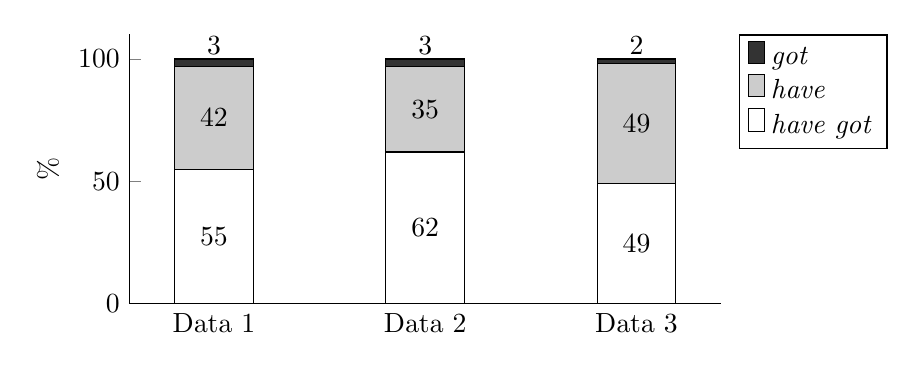
\begin{tikzpicture}
\pgfplotsset{compat=1.9}
\begin{axis}[ybar stacked,
            axis lines*=left,
			bar width=1cm,
			enlarge x limits={0.2},
			height=5cm,
			legend cell align=left,
			legend pos=outer north east,
			nodes near coords,
			reverse legend,
			symbolic x coords={Data 1,Data 2,Data 3},
			width=.75\textwidth,
            xtick=data,
			ylabel=\%,
			ymin=0,
			]
	\addplot [fill=white,draw=black] coordinates {(Data 1,55) (Data 2,62) (Data 3,49)};
	\addlegendentry{\textit{have got}}
	\addplot [fill=black!20, draw=black] coordinates {(Data 1,42) (Data 2,35) (Data 3,49)};
	\addlegendentry{\textit{have}}
	\addplot [fill=black!80, draw=black, nodes near coords bar offset=1,
			   nodes near coords align={above, yshift=-2pt}] coordinates {(Data 1,3) (Data 2,3) (Data 3,2)};
	\addlegendentry{\textit{got}}
\end{axis}
\end{tikzpicture}
\caption{\label{fig:hirano:1}Verbs of possession used by British speakers}
\end{figure}

However, the analysis of Data 3 suggests a reversal of the direction of this linguistic change. Compared with the results in Data 2, the use of \textit{have got} by the British speakers was lower in Data 3 (62\%→49\%), while their use of \textit{have} was higher (35\%→49\%). Further, the use of \textit{have got} in Data 3 is even lower than that in Data 1 (55\%→62\%→49\%) and the use of \textit{have} is higher than that in Data 1 (42\%→35\%→49\%). Thus, the use of \textit{have got}, which is indicative of British English characteristics, increased temporarily one year after arriving in Japan, but began to decrease in the course of their long-term stay in Japan. In contrast, the use of \textit{have}, which is characteristic of American English, decreased \textit{temporarily} one year after arriving in Japan, but then began to increase.

\begin{table}
\begin{tabularx}{.66\textwidth}{X rr rr@{}l rr}
\lsptoprule
 & \multicolumn{2}{c}{Data 1} & \multicolumn{3}{c}{Data 2} & \multicolumn{2}{c}{Data 3}\\
\cmidrule(lr){2-3}
\cmidrule(lr){4-6}
\cmidrule(lr){7-8}
Variant              &  n &  \%    &  n &  \%    &    &  n &  \%\\\midrule
\textit{must}        &  8  &  10\% &  2  &  2\%  &    &  0 &  0\%\\
\textit{have got to} &  20 &  24\% &  52 &  45\% & ** &  3 &  20\%\\
\textit{have to}     &  51 &  62\% &  56 &  48\% &    &  11 &  73\%\\
\textit{got to}      &  3  &  4\%  &  6  &  5\%  &    &  1 &  7\%\\
\lspbottomrule
\end{tabularx}
\caption{Verbs of obligation used by British speakers (Pearson’s Chi-Square (two-sided): ** significance at $p < 0.01$.)}
\label{tab:hirano:4}
\end{table}

\begin{figure}
% % % 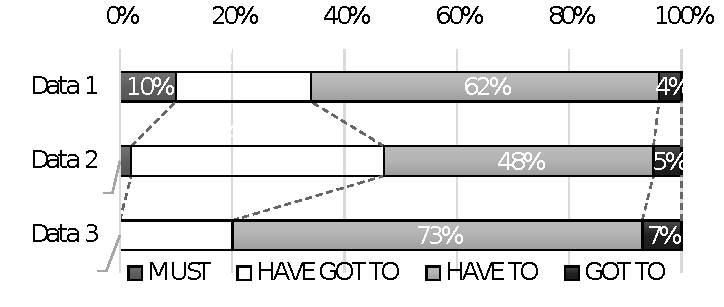
\includegraphics[width=.8\textwidth]{hirano-img002.pdf}
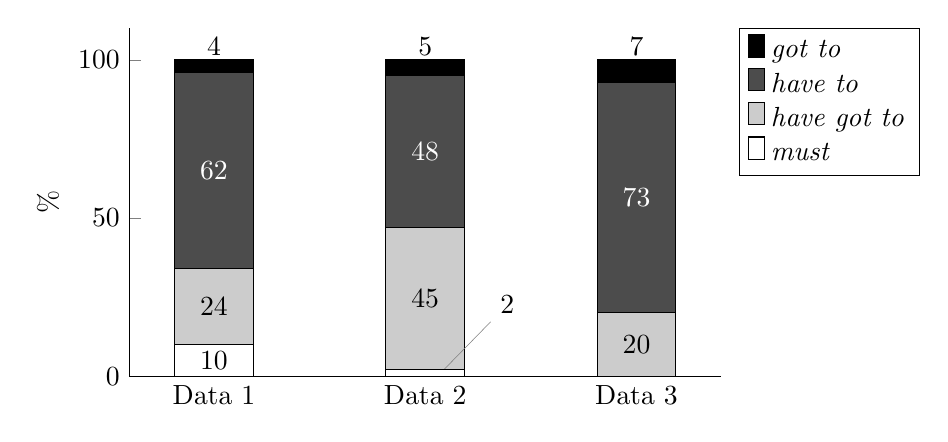
\begin{tikzpicture}
\pgfplotsset{compat=1.12}
\begin{axis}[ybar stacked,
			axis lines*=left,
			bar width=1cm,
			enlarge x limits={0.2},
			height=6cm,
			legend cell align=left,
			legend pos=outer north east,
			nodes near coords,
			reverse legend,
			symbolic x coords={Data 1,Data 2,Data 3},
			width=.75\textwidth,
            xtick=data,
			ylabel=\%,
			ymin=0,
			]
	\addplot [fill=white,draw=black,point meta=explicit symbolic] coordinates {(Data 1,10)[10] (Data 2,2)[] (Data 3,0)[]};
	\node at (axis cs:Data 2,-4) [pin={[pin distance=1cm, every pin edge/.style={shorten <=-10pt, shorten >=-10pt}]45:2}] {};
	\addlegendentry{\textit{must}}
	\addplot [fill=black!20,draw=black] coordinates {(Data 1,24) (Data 2,45) (Data 3,20)};
	\addlegendentry{\textit{have got to}}
	\addplot [fill=black!70, draw=black, text=white] coordinates {(Data 1,62) (Data 2,48) (Data 3,73)};
	\addlegendentry{\textit{have to}}
	\addplot [fill=black, draw=black, nodes near coords bar offset=1,
			   nodes near coords align={above, yshift=-2pt}] coordinates {(Data 1,4) (Data 2,5) (Data 3,7)};
	\addlegendentry{\textit{got to}}
\end{axis}
\end{tikzpicture}
\caption{\label{fig:hirano:2}Verbs of obligation used by British speakers}
\end{figure}

\tabref{tab:hirano:4} presents the distribution of verbs of obligation by British speakers, and \figref{fig:hirano:2} is the graphic form of the table. The result indicates the same tendency as verbs of possession. There was an increase in British English tendencies temporarily one year after arriving in Japan, but this decreased during their long-term stay. The analysis of Data 1 reveals that \textit{have to} was the most frequently used form (62\%), followed by \textit{have got to} (24\%), and \textit{must} (10\%), and that \textit{got to} was used only to a small extent (4\%). Further, the analysis of Data 2 reveals that there was a decreased use of \textit{have to} among British speakers from 62\% in Data~1 to 48\% in Data~2; moreover, there was an increased use of \textit{have got to} from 24\% in Data 1 to 45\% in Data 2, which is a statistically significant increase. These changes in the speakers’ choice of obligatory verbs appear to indicate that the British speakers exhibited more “Britishness” in their linguistic behaviour one year after their arrival in Japan.

However, the analysis of Data 3 indicates a backward movement in the linguistic change. The use of \textit{have got to} by the British speakers was reduced by more than half in Data 3 from that in Data 2 (45\%→20\%), while their use of \textit{have to} increased by 25\%, from 48\% to 73\%. Compared with the results in Data 1, the use of \textit{have got to} in Data 3 is actually 4\% lower (24\%→45\%→20\%) and the use of \textit{have to} is 11\% higher (62\%→48\%→73\%). These changes in the speakers’ choice of obligatory verbs from Data 1 to Data 2 and from Data 2 to Data 3 appear to indicate again, similar to the directional alteration of the linguistic change in verbs of possession, that the British speakers were inclined to exhibit more British characteristics in their linguistic behaviour after one year; however, the direction of this shift reversed, and they began to adopt the more widely used form in the course of their long-term stay in Japan.


\subsection{Distribution of variants of verbs of possession and obligation by American speakers}
\label{sec:hirano:5.2}

This section presents the distribution of variants of verbs of possession and obligation used by American speakers.  \tabref{tab:hirano:5} presents the distribution of verbs of possession used by American speakers for Data 1, 2, and 3, and  \figref{fig:hirano:3} is the graphic form of the table. The analysis of Data 1 reveals that \textit{have} was the most frequently used form by the American speakers (74\%), and there was less frequent usage of \textit{have got} (12\%) and \textit{got} (14\%). The analysis of Data 2 reveals that there was an increased use of \textit{have} (74\%→84\%) among the American speakers and a decreased use of \textit{got} (14\%→4\%) with statistical significance, while their use of \textit{have got} remained unchanged (12\%→12\%). In other words, Americans neither increased nor decreased their use of the British-English feature, maintaining more typically “American” constructions a year later.

\begin{table}
\begin{tabular}{l rr rr@{}l rr@{}l}
\lsptoprule
  & \multicolumn{2}{c}{Data 1} & \multicolumn{3}{c}{Data 2} & \multicolumn{3}{c}{Data 3}\\\cmidrule(lr){2-3}\cmidrule(lr){4-6}\cmidrule(lr){7-9}
Variant           &  n  &  \%   &  n   &  \%   &    &   n &  \%   & \\\midrule
\textit{have got} &  13 &  12\% &  15  &  12\% &    &  20 &  19\% & \\
\textit{have}     &  79 &  74\% &  104 &  84\% &    &  79 &  73\% & *\\
\textit{got}      &  15 &  14\% &  5   &  4\%  & ** &  9  &  8\%  & \\
\lspbottomrule
\end{tabular}
\caption{Verbs of possession used by American speakers (Pearson’s Chi-Square (two-sided): ** significance at $p < 0.01$; * significance at $p < 0.05$.)}
\label{tab:hirano:5}
\end{table}

\begin{figure}
% % % 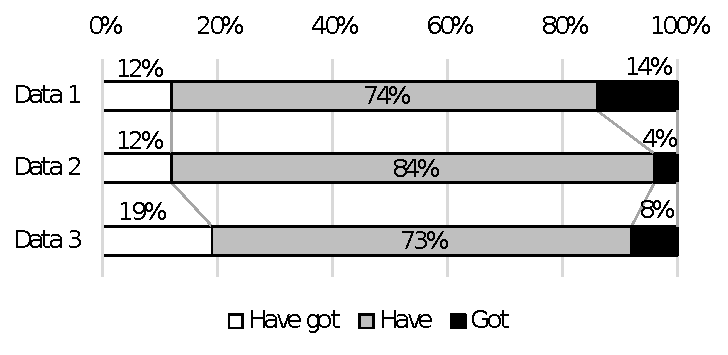
\includegraphics[width=.8\textwidth]{hirano-img003.pdf}
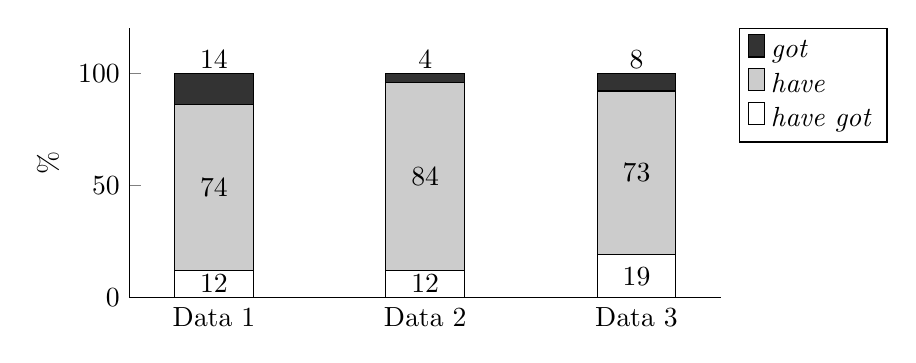
\begin{tikzpicture}
\pgfplotsset{compat=1.12}
\begin{axis}[ybar stacked,
			axis lines*=left,
			bar width=1cm,
			enlarge x limits={0.2},
			enlarge y limits={upper,value=0.2},
			height=5cm,
			legend cell align=left,
			legend pos=outer north east,
			nodes near coords,
			reverse legend,
			symbolic x coords={Data 1,Data 2,Data 3},
			width=.75\textwidth,
            xtick=data,
			ylabel=\%,
			ymin=0,
			]
	\addplot [fill=white,draw=black] coordinates {(Data 1,12) (Data 2,12) (Data 3,19)};
	\addlegendentry{\textit{have got}}
	\addplot [fill=black!20, draw=black] coordinates {(Data 1,74) (Data 2,84) (Data 3,73)};
	\addlegendentry{\textit{have}}
	\addplot [fill=black!80, draw=black, nodes near coords bar offset=1, 
			   nodes near coords align={above, yshift=-2pt}] coordinates {(Data 1,14) (Data 2,4) (Data 3,8)};
	\addlegendentry{\textit{got}}
\end{axis}
\end{tikzpicture}
\caption{Verbs of possession used by American speakers}
\label{fig:hirano:3}
\end{figure}

However, when the result of the analysis of Data 3 was compared with that of Data 2, the American speakers’ use of \textit{have} was found to be lower (84\%→73\%) with statistical significance, while their use of \textit{have got} was higher (12\%→19\%). Thus, the percentage use of \textit{have got}, which is characteristic of British English, did not change from the time they arrived in Japan to one year later but increased during their long\hyp term stay in Japan (12\%→12\%→19\%). The combined percentage use of \textit{have} and \textit{got}, which are typical features of American English, also remained unchanged for a year, but subsequently began to decrease (88\% → 88\% → 81\%).

\tabref{tab:hirano:6} presents the distribution of verbs of obligation by American speakers, and \figref{fig:hirano:4} is the graphic form of the table. The distribution reveals a slightly different tendency from that of verbs of possession. American speakers adopted British English characteristics only to a small extent one year later, but this increased in the course of their long-term stay in Japan. The analysis of Data 1 indicates that \textit{have to} was the most frequently used form (81\%), followed by \textit{got to} (16\%) and \textit{must} (3\%); however, \textit{have got to} was not used at all. The analysis of Data 2 reveals that there was a slight decrease of the use of \textit{have to} from 81\% in Data 1 to 71\% in Data 2 among American speakers and an increase in their use of \textit{got to} from 16\% in Data 1 to 22\% in Data 2. The use of \textit{have got to} increased from null in Data 1 to 5\% in Data 2, but the use of \textit{must} slightly reduced from 3\% in Data 1 to 2\% in Data 2. The combined percentage use of \textit{have to} and \textit{got to}, which are characteristic of American English, slightly decreased from 97\% to 93\%, while the combined percentage use of \textit{have got to} and \textit{must}, which are typical features of British English, slightly increased from 3\% to 7\%.

\begin{table}
\begin{tabularx}{.66\textwidth}{X rr rr rr}
\lsptoprule
& \multicolumn{2}{c}{Data 1} & \multicolumn{2}{c}{Data 2} & \multicolumn{2}{c}{Data 3}\\\cmidrule(lr){2-3}\cmidrule(lr){4-5}\cmidrule(lr){6-7}
Variant &  n &  \% &  n &  \% &  n &  \%\\
\midrule
\textit{must} &  2 &  3\% &  1 &  2\% &  0 &  0\%\\
\textit{have got to} &  0 &  0\% &  3 &  5\% &  7 &  16\%\\
\textit{have to} &  51 &  81\% &  43 &  71\% &  34 &  79\%\\
\textit{got to} &  10 & \multicolumn{1}{c}{ 16\%} &  13 &  22\% &  2 &  5\%\\
\lspbottomrule
\end{tabularx}
\caption{Verbs of obligation used by American speakers}
\label{tab:hirano:6}
\end{table}


\begin{figure}
% 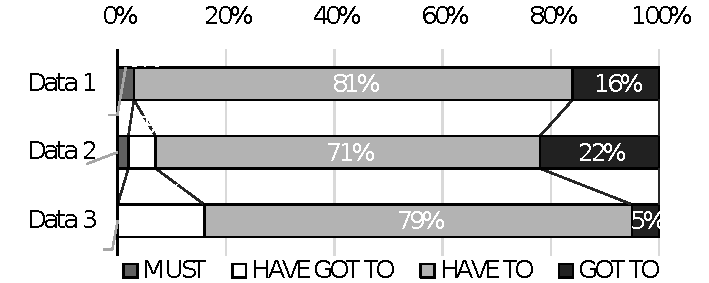
\includegraphics[width=.8\textwidth]{hirano-img004.pdf}
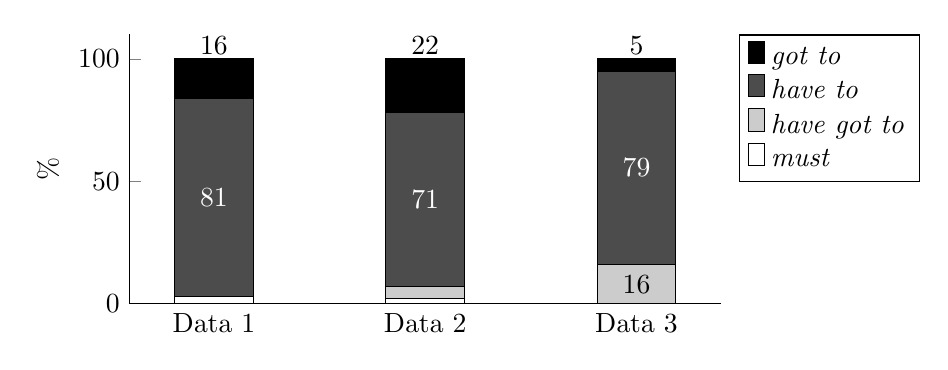
\begin{tikzpicture}
\pgfplotsset{compat=1.12}
\begin{axis}[ybar stacked,
			axis lines*=left,
			bar width=1cm,
			enlarge x limits={0.2},
			height=5cm,
			legend cell align=left,
			legend pos=outer north east,
			nodes near coords,
			reverse legend,
			symbolic x coords={Data 1,Data 2,Data 3},
			width=.75\textwidth,
            xtick=data,
			ylabel=\%,
			ymin=0,
			]
	\addplot [fill=white,draw=black,point meta=explicit symbolic] coordinates {(Data 1,3)[] (Data 2,2)[] (Data 3,0)[]};
	\addlegendentry{\textit{must}}
	\addplot [fill=black!20,draw=black,point meta=explicit symbolic] coordinates {(Data 1,0)[] (Data 2,5)[] (Data 3,16)[16]};
	\addlegendentry{\textit{have got to}}
	\addplot [fill=black!70, draw=black, text=white] coordinates {(Data 1,81) (Data 2,71) (Data 3,79)};
	\addlegendentry{\textit{have to}}
	\addplot [fill=black, draw=black, nodes near coords bar offset=1,
			   nodes near coords align={above, yshift=-2pt}] coordinates {(Data 1,16) (Data 2,22) (Data 3,5)};
	\addlegendentry{\textit{got to}}
\end{axis}
\end{tikzpicture}
\caption{Verbs of obligation used by American speakers}
\label{fig:hirano:4}
\end{figure}

The analysis of Data 3 indicates a further decrease in the use of forms associated with American English and a further increase in the use of forms characteristic of British English. The use of \textit{have to} by the American speakers increased from 71\% in Data 2 to 79\% in Data 3, but their use of \textit{got to} notably reduced from 22\% in Data 2 to 5\% in Data 3. The combined percentage use of \textit{have to} and \textit{got to} decreased from 93\% in Data 2 to 84\% in Data 3. In contrast, the use of \textit{have got to} increased from 5\% in Data 2 to 16\% in Data 3, although \textit{must} was no longer used. Further, the changes in the speakers’ choice of obligatory verbs from Data 1 to Data 2 were somewhat small, while these changes were rather noticeable from Data 2 to Data 3. This indicates that the level of linguistic changes does not remain stable, but may advance further with the progression of time. 





\section{Discussion and conclusion} %6. /
\label{sec:hirano:6}

The analysis and comparison of the three corpora indicate that the linguistic change in the dialect contact environment in Japan does not necessarily take place unidirectionally but may shift over time. One linguistic process that occurs in the formation of new dialects in a dialect contact environment is “levelling” (\cites[149--150]{Britain2018}[98--102]{Trudgill1986})~--  a phenomenon in which marked or minority variants gradually disappear and unmarked or majority variants tend to survive in the dialect mixture. The nationality of the largest number of NSsE living in Japan is American (\citealt{eStat2021}). If the proportion of American residents among the total number of NSsE in Japan is considered, \textit{have} and \textit{have to} should be the most commonly used form of possessive and obligatory verbs. Indeed, \textit{have} and \textit{have to} are the most frequently used forms among British and American residents in Japan, and the proportions of the use of \textit{have} and \textit{have to} among these speakers have, in fact, slightly increased from Data 1 to Data 3. However, the proportions of the use of \textit{have got} and \textit{have got to} among these speakers in Data 3 did not decrease from that in Data 1. Further, the proportion of the use of \textit{have got} among these speakers in Data 3 was preserved at almost the same level as that in Data 1, and the proportion of the use of \textit{have got to} actually increased in Data 3. Therefore, there was no strong evidence of levelling in terms of the use of verbs of possession and obligation observed in Japan.

One year after arriving in Japan, British speakers showed more British English characteristics in the use of both verbs of possession and obligation. American speakers maintained the same level of American English characteristics in the use of verbs of possession as when they had arrived in Japan, but there was a slight decrease in terms of the use of verbs of obligation. However, there appeared to be a shift in the direction of linguistic change in the course of their long-term stay in Japan. Further, there was an increased use of \textit{have} and \textit{have to} among British speakers~– both of which have a strong association with American English~– at some point after a year of living in Japan. On the other hand, the American speakers began to increasingly use \textit{have got} and \textit{have got to}, which have a strong association with British English, thereby reducing the effect of the American English characteristic.

These linguistic changes appear to be the outcome of “long-term accommodation” \citep[11--21]{Trudgill1986} in which speakers adopt certain linguistic features in another variety of the same language and incorporate these features permanently. According to research which investigated long-term speech accommodation in adults who had moved from one dialect region to another, the language of these adults tended to be modified to eliminate the linguistic features of the old dialect and adopt the linguistic features of the new dialect (\citealt{EvansIverson2007, Kerswill1993, Nycz2011, Omdal1994, Shockey1984, Stanford2008}). In Japan, English is not the primary language among the local citizens and, therefore, there is no single target English dialect which the NSsE are expected to assimilate. However, in the Anglophone community in Japan, which is the focus of the current research, both British and American speakers come in contact with different varieties and dialects of the English language while living in Japan on a daily basis. They do not appear to accommodate each other’s linguistic features of grammatical aspects immediately after their encounter with other English dialects or during the early stages of the mixing of dialects; however, eventually they appear to begin to adopt each other’s linguistic features. As far as the findings of the current study are concerned, the speed of linguistic accommodation differs depending on which variety of English the speakers modify and which variety of English they adopt. The American speakers appeared to begin adapting to the different variety of English earlier than the British speakers in this study.

In conclusion, the present study attempted to address the different stages of long-term accommodation by reporting the outcomes of analyses of three sets of corpora in a real-time study on dialect contact and grammatical variation in a community in which no single dominant variety or regional dialect of English exists. It is important to continue to monitor the change in the linguistic characteristics of individual speakers in order to explore the complexity of the mechanisms of linguistic change in English due to dialect contact in Japan. Once additional linguistic data from a greater variety of speakers are collected, further statistical analyses must be conducted in various possible aspects in order to unfold new findings and validate the outcomes.

\section*{Acknowledgment}

This work was supported by JSPS KAKENHI Grant Number 26370494.

\printbibliography[heading=subbibliography,notkeyword=this]
\end{document}
